\documentclass{ctexbook}
\usepackage[T1]{fontenc}
\usepackage[a4paper,top=1.5cm,bottom=1.5cm,left=2cm,right=2cm,marginparwidth=1.75cm]{geometry}
\usepackage{mathtools}
\usepackage{tikz}
\usepackage{booktabs}
\usepackage{caption}
\usepackage{outlines}
\usepackage{graphicx}
\usepackage{float}
\usepackage{amsthm}
\usepackage{tabularray}
\usepackage{minted}
\usepackage[colorlinks=false, allcolors=blue]{hyperref}
\usepackage{cleveref}
\usetikzlibrary{fit}
\usetikzlibrary{calc}
\usetikzlibrary{arrows}
\usetikzlibrary{positioning}
\renewcommand{\tableautorefname}{表}
\DeclarePairedDelimiter{\set}{\{}{\}}
\DeclarePairedDelimiter{\paren}{(}{)}
\graphicspath{ {./images/} }

\newcounter{fullrefcounter}
\newcommand*{\fullref}[1]{%
\addtocounter{fullrefcounter}{1}%
\label{--ref-\thefullrefcounter}%
\ifthenelse{\equal{\getpagerefnumber{--ref-\thefullrefcounter}}{\getpagerefnumber{#1}}}
  {
    \hyperref[{#1}]{\Cref*{#1} \nameref*{#1}}
  }
  {% false case
    \hyperref[{#1}]{第 \pageref*{#1} 页 \Cref*{#1} \nameref*{#1}}
  }
}

\title{软件工程引论课程笔记}
\author{卢雨轩 19071125}
% \date{\today}
\ctexset{
    section = {
        titleformat = \raggedright,
        name = {,},
        number = \chinese{section}、
    },
    paragraph = {
        runin = false
    },
    today = small,
    figurename = 图,
    contentsname = 目录,
    tablename = 表,
}

\begin{document}

\maketitle

\chapter{软件工程概述}
\section{软件的生存期模型}
\subsection{瀑布模型}
\begin{figure}[!htp]
    \centering
    \begin{tikzpicture}[
        every node/.append style={draw=black,text width=2cm, align=center}
    ]
        \node (1) [] {可行性分析}; 
        \node (2) [below right= .5cm and -.6cm of 1] {需求分析};
        \node (3) [below right= .5cm and -.6cm of 2] {概要设计};
        \node (4) [below right= .5cm and -.6cm of 3, dashed] {详细设计};
        \node (5) [below right= .5cm and -.6cm of 4,dashed] {编码};
        \node (6) [below right= .5cm and -.6cm of 5,dashed] {测试};
        \node (7) [below right= .5cm and -.6cm of 6,dashed] {交付};
        \node (8) [below right= .5cm and -.6cm of 7,dashed] {维护};
    
        \node (9) [right=2cm of 2] {变化的需求};

        \draw (1) -| (2);
        \draw (2) -| (3);
        \draw (3) -| (4);
        \draw (4) -| (5);
        \draw (5) -| (6);
        \draw (6) -| (7);
        \draw (7) -| (8);

        \draw [-latex,dashed] ([xshift=.4cm]8.north) |- (9);
        \draw [-latex,dashed] (9) -| ([xshift=.2cm]3.north);
        \draw [-latex,dashed] ([xshift=.3cm]8.north) |- ([yshift=1.5mm]4.east);
        \draw [-latex,dashed] ([xshift=.2cm]8.north) |- ([yshift=1.5mm]5.east);
        \draw [-latex,dashed] ([xshift=.1cm]8.north) |- ([yshift=1.5mm]6.east);
    \end{tikzpicture}
    \caption{软件工程的瀑布模型}
    实线表示开发过程,虚线表示维护过程
\end{figure}
特点:线性,不适应需求变化

\section{快速原型模型}
\begin{outline}
    \1 快速的开发一个原型软件
    \1 展示给客户并征求意见,逐步完善
    \1 强调快速
    \1 优点:
        \2 有助于满足用户的真实需求
        \2 规格说明文档能够正确的描述用户需求
        \2 软件开发基本按照线性顺序进行
        \2 开发过程的后续阶段不会因为发现规格文档的错误而进行较大的反工
    \1 缺点:
        \2 过程不可见
        \2 系统结构较差
        \2 特殊工具和技术的使用
\end{outline}

\section{增量模型}

\begin{figure}[!htp]
    \centering
    \begin{tikzpicture}[
        every node/.append style={draw=black,text width=2cm, align=center,rounded corners},
        every path/.append style={-latex}
    ]
        \node (1) {定义基本需求};
        \node (2) [right=1cm of 1] {将需求对应到各增量};
        \node (3) [right=1cm of 2] {设计系统架构};
        \node (4) [below right=1cm and .5cm of 1] {开发其中一个增量};
        \node (5) [right=1cm of 4] {检验和确认该增量};
        \node (6) [right=1cm of 5] {将增量集成到系统中};
        \node (7) [right=1cm of 6] {确认集成后的系统};

        \draw (1) -- (2);
        \draw (2) -- (3);
        \draw (3.east) -- ++(1,0) -- ++(0,-1) -- ++(-8,0) |- (4.west);
        \draw (4) -- (5);
        \draw (5) -- (6);
        \draw (6) -- (7);
        \draw (7) -- ++(0,-1.3) -| (4);
        \draw (7) -- ++(2, 0);
    \end{tikzpicture}
\end{figure}

\section{统一过程}

\begin{figure}[htp]
    \centering
    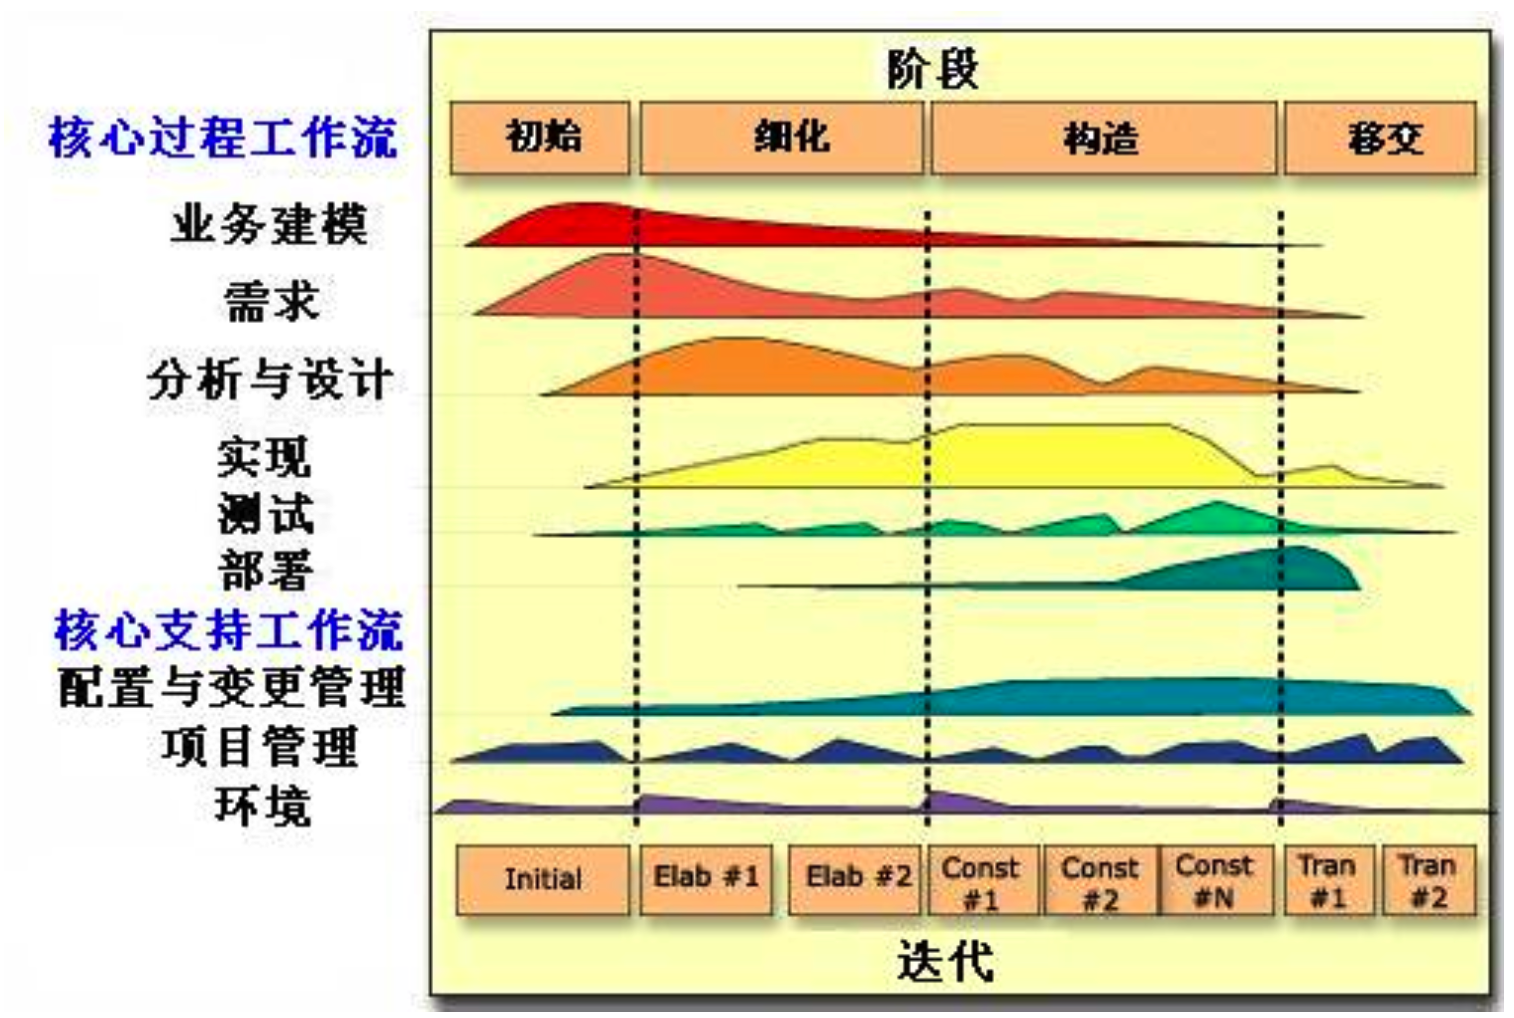
\includegraphics[width=.8\linewidth]{image1.png}
    \caption{软件开发的统一过程}
\end{figure}

\begin{outline}
    \1 占领市场
    \1 频繁发布
    \1 频繁更新
    \1 需要注意的问题:
        \2 必须不破坏已经开发的产品
        \2 体系结构必须开放
        \2 最重要的系统服务要接受最多的测试
        \2 需要更精心的设计
\end{outline}

\section{测试}
\begin{outline}
    \1 测试用例:
        \2 输入,预期结果,实际结果
        \2 设计,执行
    \1 测试的种类
        \2 系统测试
            \3 整个系统,执行和设计
        \2 集成测试
            \3 测试模块之间的集成
        \2 单元测试
            \3 每个单元的功能的正确性
\end{outline}

\end{document}
